\subsection{Спектральные классы звёзд}
\begin{table}[h!]
    \centering
    \footnotesize
    \renewcommand{\arraystretch}{1.4}
    \renewcommand{\tabcolsep}{0pt}
    \begin{tabularx}{\tw}{|C{0.1}|C{0.3}|C{0.23}|C{0.13}|C{0.13}|C{0.13}|}
        \hline
        {\bfseries Класс} & {$\mathbf{T}$, К} & {\bfseries Цвет} & {$\mathbf{M}$, $M_{\odot}$} & {$\mathbf{R}$, $R_{\odot}$} & {$\mathbf{L}$, $L_{\odot}$}\\
        \hline
        O & $3 \times 10^4$ --- $6 \times 10^4$ & Голубой & 60 & 15 & $1.4 \times 10^6$\\

        B & $1 \times 10^4$ --- $3 \times 10^4$ & Бело-голубой & 18 & 7 & $2 \times 10^4$\\

        A & $7.5 \times 10^3$ --- $1 \times 10^4$ & Белый & 3.1 & 2.1 & 80\\

        F & $6 \times 10^3$ --- $7.5 \times 10^3$ & Жёлто-белый & 1.7 & 1.3 & 6\\

        G & $5 \times 10^3$ --- $6 \times 10^3$ & Жёлтый & 1.1 & 1.1 & 1.2\\

        K & $3.5 \times 10^3$ --- $5 \times 10^3$ & Оранжевый & 0.8 & 0.9 & 0.4\\

        M & $2 \times 10^3$ --- $3.5 \times 10^3$ & Красный & 0.3 & 0.4 & 0.04\\
        \hline
    \end{tabularx}
    \caption{Современная спектральная классификация звёзд}
    \label{tab:spectr-types}
\end{table}
Звёзды в зависимости от своего цвета делятся на \imp{спектральные классы}, основные из них представлены в Таблице\,\ref{tab:spectr-types}. Масса, радиус и светимость приведены средних представителей спектрального класса, лежащих на главной последовательности (V).

Запись спектрального класса представляет собой латинскую букву, арабское число и римское число, например, спектральный класс Солнца~--- G2V. арабское число показывает к какой именно части спектрального класса относится звезда: к более синей (число меньше) или к красной (число больше). Так,~G10V~--- это тоже самое, что K0V. Спектральный класс (показатель цвета) и абсолютная звёздная величина задают положение звезды на \imp{Диаграмме Герцшпрунга-Рассела}.


%    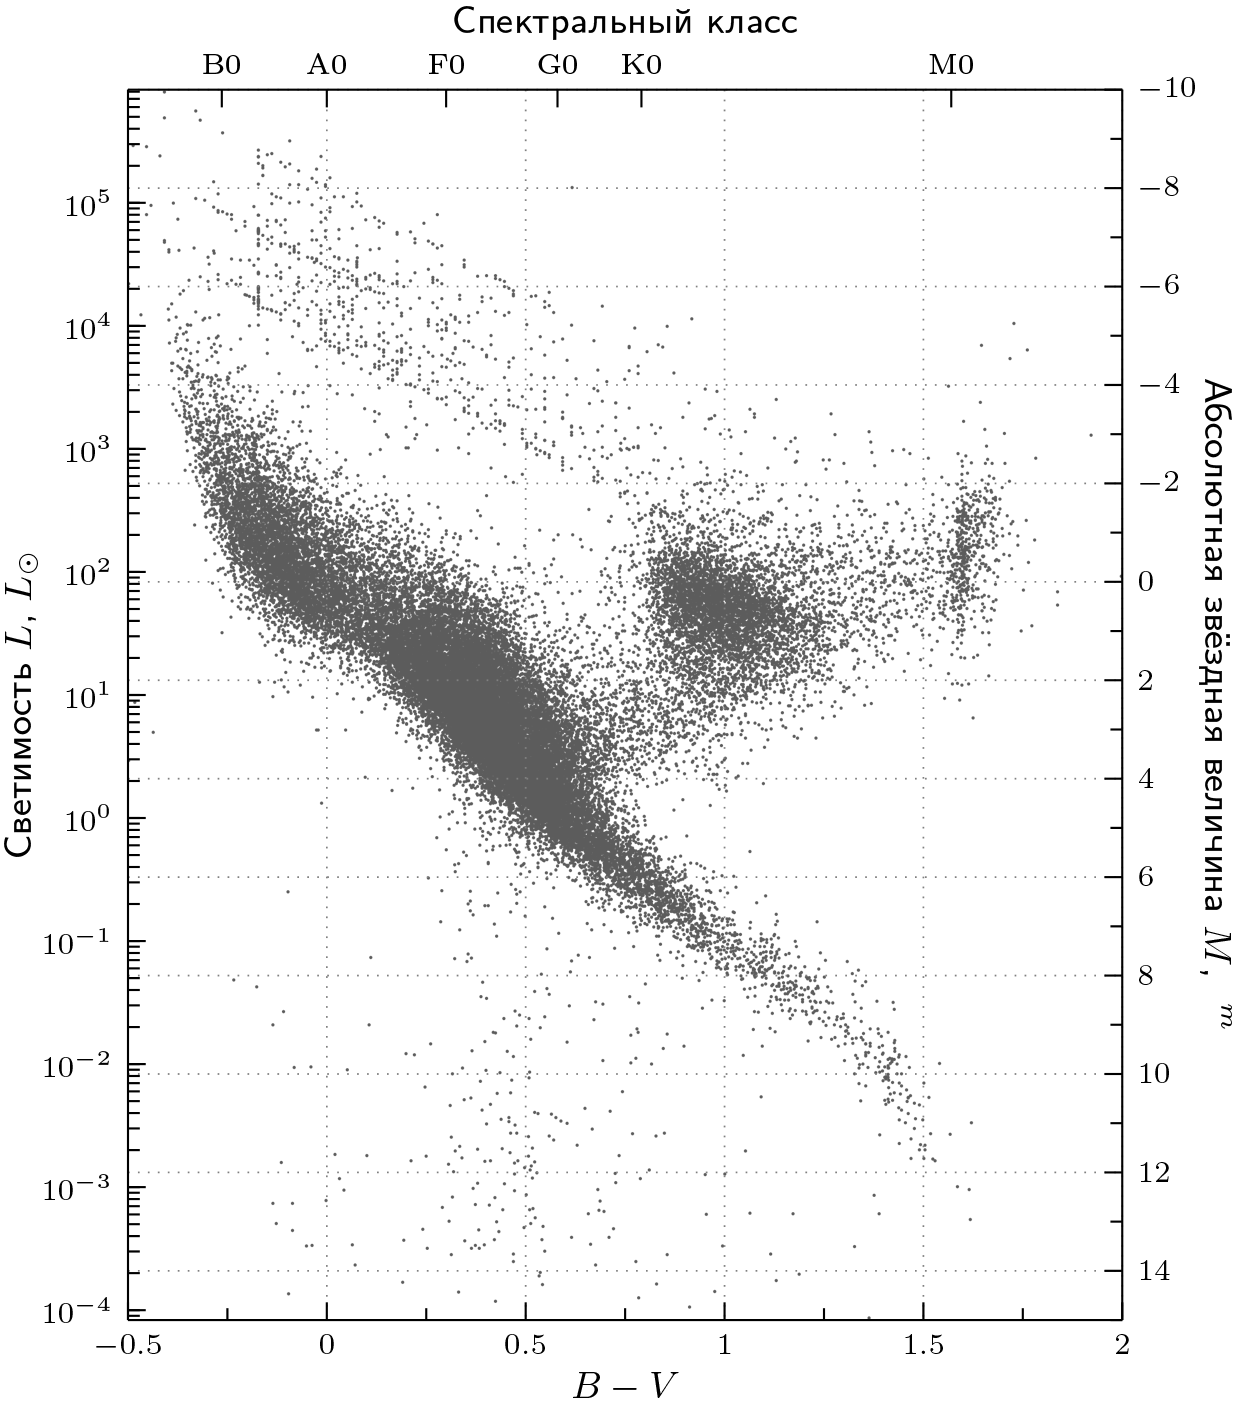
\includegraphics[width=10cm]{gr}

\term{Диаграмма Герцшпрунга-Рассела} показывает зависимость светимости или абсолютной звёздной величины от спектрального класса, показателя цвета $(B-V)$ или эффективной температуры фотосферы звезды.

Была предложена примерно в 1910 году независимо Эйнаром Герцшпрунгом и Генри Расселом. Диаграмма используется для классификации звёзд и соответствует современным представлениям о звёздной эволюции.

Около $90 \%$ звёзд находятся на главной последовательности. Их светимость обусловлена термоядерными реакциями превращения водорода в гелий. Выделяется также несколько ветвей проэволюционировавших звёзд-гигантов, в которых происходит горение гелия и более тяжёлых элементов. В левой нижней части диаграммы находятся полностью проэволюционировавшие белые карлики.

Мнемонические правила для запоминания спектральных классов: <<\textbf{O}h \textbf{B}e \textbf{A} \textbf{F}ine \textbf{G}irl, \textbf{K}iss \textbf{M}e \textbf{R}ight \textbf{N}ow \textbf{S}weetheart.>> и <<\textbf{В}ообразите: \textbf{О}дин \textbf{Б}ритый \textbf{А}нгличанин \textbf{Ф}иники \textbf{Ж}евал \textbf{К}ак \textbf{М}орковь --- \textbf{Р}азве \textbf{Н}е \textbf{С}мешно?>>
\begin{figure}[h!]
    \centering
    \vspace{-1pc}
    \tikzsetnextfilename{hr-diagram}
    \begin{tikzpicture}
         \begin{axis}[
                         height    =    10cm,
                         width    =    10cm,
                         ymax    =    14.,
                         ymin    =    -6.,
                         y dir    =    reverse,
                         xmax    =    2.,
                         xmin    =    -.5,
                         axis x line* = bottom,
                         axis y line* = right,
                         xlabel  =   $B-V$,
                         y label style = {at={(axis description cs: 1.07, 0.5)}, rotate=180},
                         ylabel    =    {Абсолютная звёздная величина $M$, $\!~^m$}
                     ]
            \ifthenelse{\boolean{useLightPlotVersion}}{}{
                \addplot+[only marks, mark = o, mark options={scale=0.2, darkgray}] table[x=BV, y=M]{data/gr-plot.txt};
            }
         \end{axis}
         \begin{semilogyaxis}[
                         height    =    10cm,
                         width    =    10cm,
                         ymax    =    2.088e4,
                         ymin    =    2.088e-4,
                         xmax    =    2.,
                         xmin    =    -.5,
                         minor x tick num = 0,
                         minor y tick num = 01,
                         xtick = {-0.264, 0, 0.3, 0.58, 0.791, 1.57},
                         xticklabels = {B0, A0, F0, G0, K0, M0},
                         axis x line* = top,
                         axis y line* = left,
                         xlabel    =    {Спектральный класс},
                         x label style = {at={(axis description cs: 0.5, 1.03)}, rotate=0},
                         ylabel    =    {Светимость $L$, $L_\odot$},
                         ymajorgrids     =    false,
                         xmajorgrids     =    false
                    ]
        \end{semilogyaxis}
     \end{tikzpicture}
     \caption{Диаграмма Герцшпрунга--Рассела}
    \label{}
\end{figure}
Помимо основных спектральных классов звёзд существуют дополнительные: W~--- звёзды Вольфа-Райе, очень тяжёлые яркие звёзды с температурой порядка $70000$~К и интенсивными эмиссиоными линиями спектра; L~--- звёзды или коричневые карлики с температурой 1500\,--\,2000~К и соединениями металлов в атмосфере; T~--- метановые коричневые карлики с температурой $700 - 1500$~К; Y~---  очень холодные (метано-аммиачные) коричневые карлики с температурой ниже $700$~К; C~--- углеродные звёзды, гиганты с повышенным содержанием углерода. Ранее относились к классам R и N.
